\section{Method}
\subsection{Antenna orientation}
The relative antenna orientation between receiver-transmitter pairs is a major factor in signal strength variability, even in the absence of multipath and shading effects\cite{lymberopoulos2006ecr}. This is due to the fact that antenna's are not perfectly omnidirectional. Ideally, the radiation pattern of an antenna should be uniform and it should look like a circle (2-D space) or a sphere (3-D space). However, in practice, the orientation of the antenna can influence the signal strength by several decibels. Thus, different antenna orientations can produce different sets of RSS values for the same distances between receiver and transmitter, increasing the position error.

Therefore, it is imperative that the antenna's orientation should be accounted for as well. One possible solution would to use a compass to determine the nodes orientation. Given the antennas radiation pattern the transmitted power can easily be obtained. 

A straightforward solution would be to use a more omnidirectional antenna to minimize these effects. For example, Telos rev.B nodes use an onboard antenna. The power received from this antenna can differ by as much as 20dB depending on the orientation.  Fortunately, an external antenna is supported. This can be mounted on the circuit board via an optional standard SMA connector. 

We tested the difference between a node employed with and without an external antenna.

\subsubsection{Set up}
Two Telos rev. B nodes were set in an obstacle-free environment (basketball court). 
The test exists out of two parts:
In the first part, the two nodes are equipped with an external antenna with a gain of 6dBi and placed at a distance of one meter and at a distance of five meters from each other at a height of one meter. This way the ground will not absorb or weaken the signal. One node is set as an anchor node and will broadcast beacon messages at a rate of 200 ms. The anchor node was rotated and samples were taken at every 20 degrees. The other node, the blind node sends the RSSI to the database. Approximately 25 samples were collected at every orientation.

In the second part, only one node is equipped with the external antenna and placed at a distance of one and five meter. This node is set as the blind node and receives ideally the same power in every direction. The other node with an integrated antenna is the anchor node that will broadcast. 

\subsubsection{Results}
\begin{figure}[h]
	\centering
		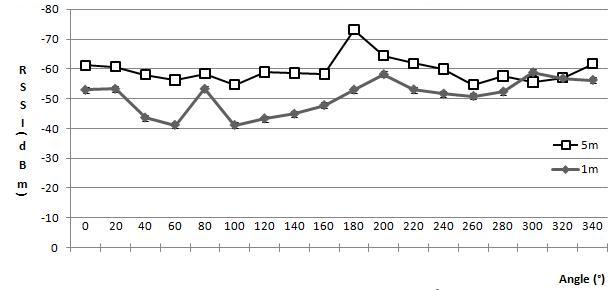
\includegraphics[scale=0.51]{Images/1and5mwithoutantenna.jpg}
	\caption{Average RSSI at a distance of 1m and 5m with one node equiped with an external antenna}
	\label{fig:1and5mnoa}
\end{figure}

\begin{figure}[h]
	\centering
		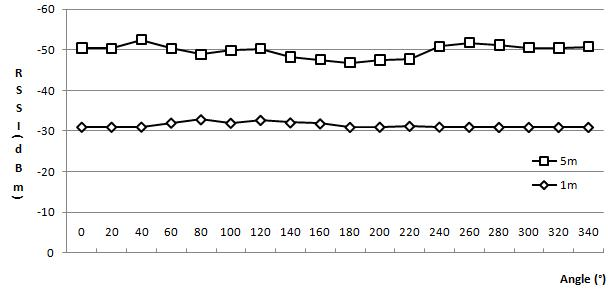
\includegraphics[scale=0.51]{Images/1and5mwithantenna.jpg}
	\caption{Average RSSI at a distance of 1m and 5m with the two nodes equiped with an external antenna}
	\label{fig:1and5mwoa}
\end{figure}

\begin{table}[ht]
\caption{Table with average RSSI and standard deviation}
\label{table:resultsorient}
\centering
\begin{tabular}{|l|l|l|l|} \hline
\multicolumn{4}{|c|}{Results} \\ \hline
\multirow{} & Average & Stdv1 & Stdv2 \\ \hline
\multirow{Onboard antenna at one meter} & -50,65 & 1,144 & 5,71 \\ \hline
\multirow{Onboard antenna at five meter} & -59,50 & 1,63 & 4,31 \\ \hline
\multirow{External antenna at one meter} & -31,46 & 0,21 & 0,64 \\ \hline
\multirow{External antenna at five meter} & -49,77 & 0,90 & 1,61 \\ \hline
\end{tabular}
\end{table}

Figure \ref{fig:ExternalAntenna} and \ref{fig:OnboardAntenna} display the mean and standard deviation of the RSS when rotating the node. Table \ref{table:resultsorient} displays the average standard deviation for each orientation and the standard deviation of the entire dataset. Note that the standard deviation is sometimes too small to be seen on the graph. These results show that RSS readings are more stable when the node is equipped with a more omnidirectional antenna. However the readings with onboard antenna are fairly stable as well. The results also clearly show that the external antenna is more invariant to orientation than the onboard antenna. 
The results are consistent with the common belief that node orientation influences RSS readings.

\subsection{In \& outdoor positioning}
In this section, we will test the accuracy and thus the position error of our 2 range-based algorithms namely Min-Max and multilateration.

\subsubsection{Set up}
We placed a total of 10 nodes in an obstacle-free environment. Nine of them are configured as anchor node and the last one as a blind node. All the nodes are placed at a height of one meter.
The anchor nodes are placed randomly at fixed locations (in meters):
\begin{itemize}
	\item Node one: 1.19  ; 6.98
	\item Node two: 2.00 ; 8.48
	\item Node three: 3.00 ; 1.50
	\item Node four: 3.19 ; 6.23
	\item Node five: 1.19 ; 5.14
	\item Node six: 4.64 ; 3.88
	\item Node seven: 4.67 ; 0.00
	\item Node eight: 2.50 ; 0.00
	\item Node nine: 0.00 ; 0.00
\end{itemize}
The blind node will be located at the following locations (in meters):
\begin{enumerate}
	\item 5.07 ; 8. 48
	\item 5.07; 4.63
	\item 2.00 ; 1.50
	\item 0.00 ; 3.29
	\item 3.19 , 6.23
	\item 1.19 , 8.48
\end{enumerate}
\subsubsection{Results}